
This chapter will describe all the development tools and infrastructure used. Besides, it includes a brief description of the kick engine which this work was based on, and the set of metrics we will use to evaluate our learning results and performance.

\section{Tools}

\subsection{C++}

C++ is a general purpose programming language that is highly efficient and flexible. It is famous for introducing a oriented-based paradigm with high performance processing, by allowing low-level memory manipulations and a machine compiled syntax. \cite{C++}

The ITAndroids Soccer3D base code was already built in C++, and therefore any additional work made which interacts with the soccer simulation server was also developed in C++ in order to integrate seamlessly with the codebase. For this work, we used version 14, which is one of the most recent and stable standardized version.

\subsection{Python}

Python is an interpreted general purpose high-level programming language \cite{Python}. It has a easy-to-read syntax closely resembling pseudo-code, which makes easier and quicker to prototype new ideas and develop. For this reason, Python was widely chosen as one of the most used programming languages in the deep learning community, and many of the AI frameworks and reference algorithms we used was developed in or have a great integration with Python.

For this work, we chose version 3.5, since it is one of the most recent and stable versions, and also is used by other frameworks.

\subsection{Protocol Buffers}

Protocol Buffers is a multiplatform library for serializing structured data that supports multiple programming languages \cite{ProtoBuf}. It is very useful for developing uncoupled client-server applications that communicate using a simple and flexible API. For these reasons, we chose Protocol Buffer as the client-server API.

\subsection{OpenAI Baselines}

OpenAI Baselines is a set of high-quality implementations of reinforcement learning algorithms open sourced by OpenAI. The purpose is to provide algorithms which will make it easier for the research community to replicate, refine, and identify new ideas, and therefore create good baselines to build research on top of. \cite{baselines}

\begin{figure}[H]
    \centering
    
\includegraphics[width=0.3\textwidth]{Chapter5/openai_logo.jpg} 
    \caption{OpenAI Logo.}
    \label{fig:openai_logo}
\end{figure}

Besides the OpenAI Baselines, we also used the OpenAI Gym, which consists of a toolkit for running reinforcement learning algorithms in different environments \cite{OpenAIGym}. It allows testing and benchmarking RL algorithms by providing a standardized set of environments. Figure \ref{fig:openai_envs} illustrates a few example environments from OpenAI Gym.

\begin{figure}[H]
    \centering
    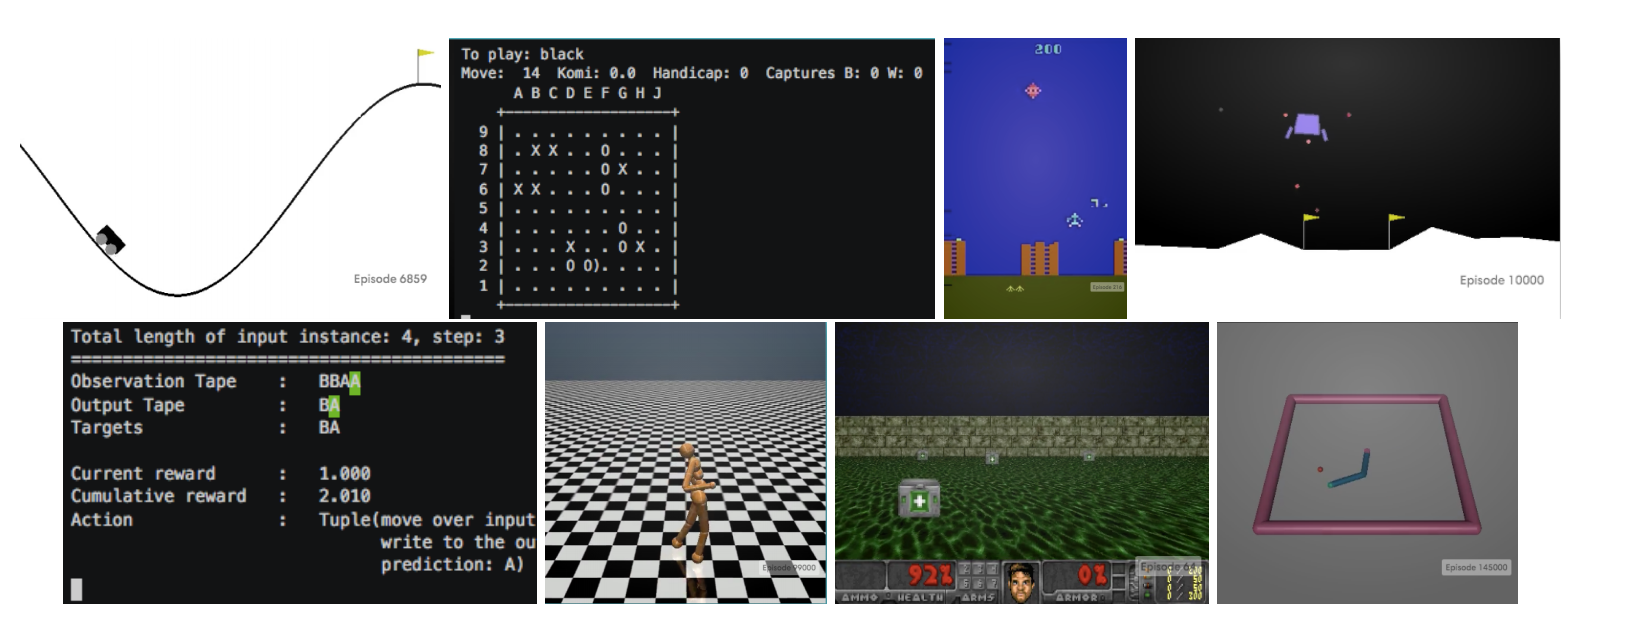
\includegraphics[width=0.85\textwidth]{Chapter5/openai_env.png} 
    \caption{OpenAI Gym environments, extracted from \cite{OpenAIGym}.}
    \label{fig:openai_envs}
\end{figure}

For these reasons, we made use of the PPO implementation from OpenAI Gym, and adapt the Gym environment to work for the Soccer3D Simulation. This process is further described in the next chapter.

\subsection{Tensorflow}

TensorFlow is an open source software library for numerical computation using data flow graph \cite{TensorFlow}. It is greatly used for machine learning applications due to its highly efficient implementations of gradient computation and optimization, by introducing parallelization and making use of specialized hardware instructions like SSE and GPU. TensorFlow is also used by OpenAI Baselines, in its RL algorithms implementations.

TensorFlow also provides several useful tools, such as TensorBoard, which consists in a visualization dashboard very helpful for debugging and plotting.

\subsection{Intel AI DevCloud}
\label{sec:devcloud}

Intel AI DevCloud is a cloud hosted hardware and software platform available to developers, researchers and startups to learn, sandbox and get started on their Artificial Intelligence Projects \cite{devcloud}. It provides access to Intel Xeon Scalable Processors, and therefore a powerful infrastructure for running optimizations and machine learning algorithms.

Intel is also a sponsor of the ITAndroids team, and provided extended use of DevCloud for this project.

\begin{figure}[H]
    \centering
    
\includegraphics[width=0.3\textwidth]{Chapter5/intelai_logo.jpg} 
    \caption{Intel AI Logo.}
    \label{fig:intelai_logo}
\end{figure}

\section{Simulation Interface}

This work's simulation environment is the \textit{SimSpark} simulator \cite{Simspark}. It makes use of the Open Dynamics Engine \cite{ODE} for rigid body dynamics and collision detection, and also allows multi-agent simulations in a single environment, hosting up to two teams of eleven humanoid robots to play against each other.

The \textit{SimSpark} server also introduces noise, breaking the reproducibility of events and turning the problem more realistic. Consequently, this process fairly increases the challenge of the learning problem.

For this work, we also used \textit{RoboViz}, a publicly available visualization tool created by Justin Stoecker \cite{RoboViz} that allows several improvements over the default visualization tool. Figure \ref{fig:roboviz_game} shows a typical game scene inside \textit{RoboViz}.

\begin{figure}[H]
    \centering
    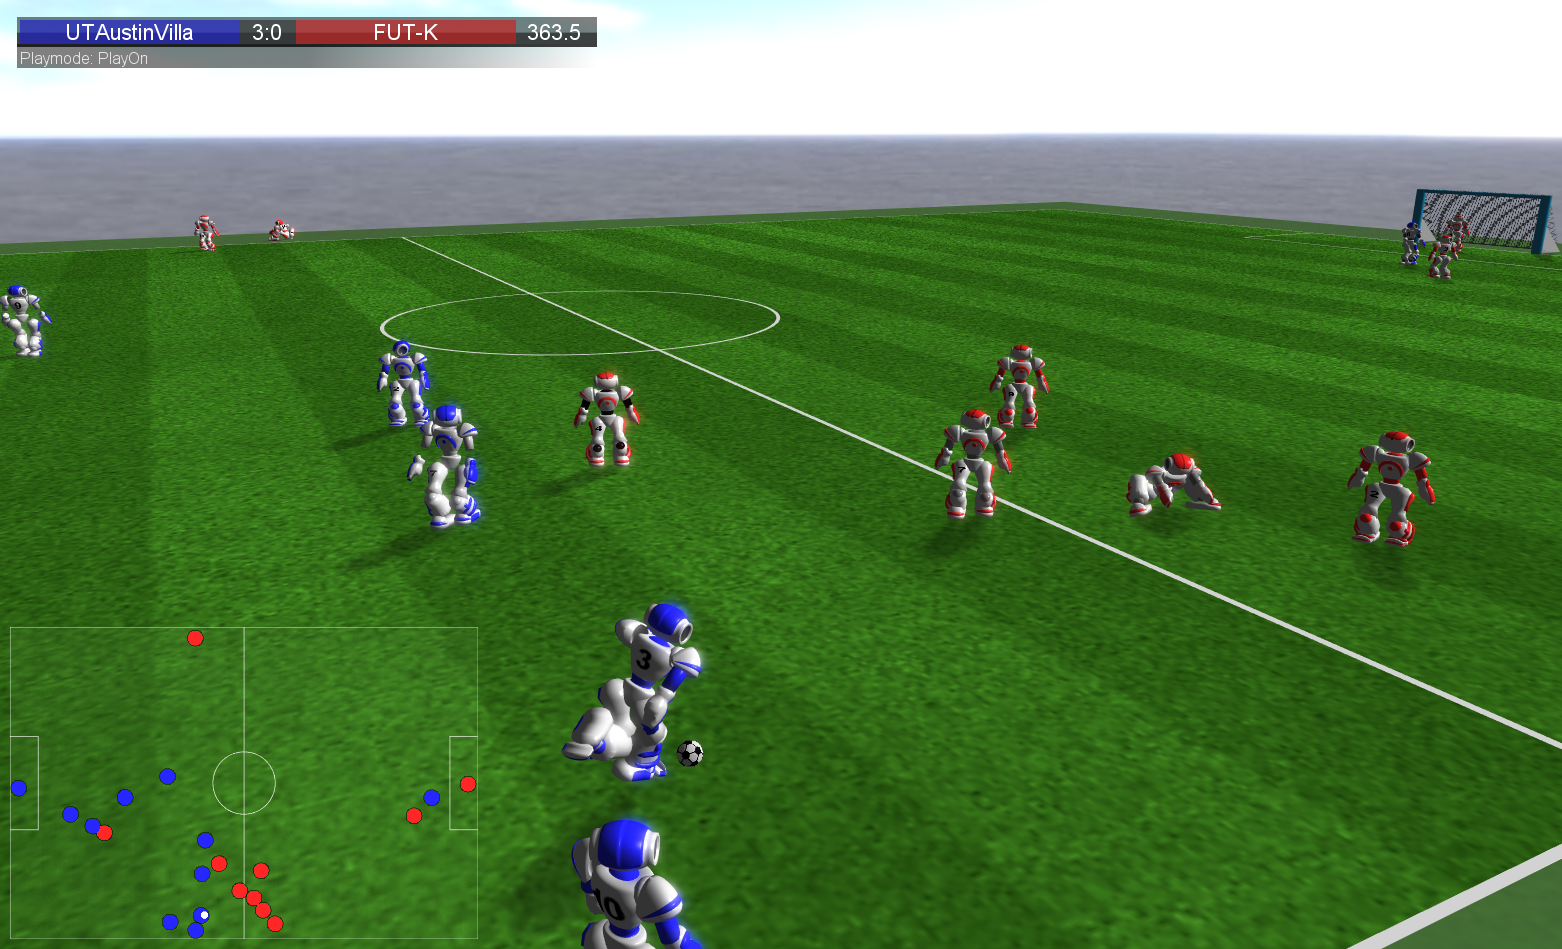
\includegraphics[width=0.8\textwidth]{Chapter5/sim3d.png} 
    \caption{Soccer match in \textit{SimSpark} simulation environment.}
    \label{fig:roboviz_game}
\end{figure}

The agent in \textit{SimSpark} is a simulated version of the Nao humanoid robot, manufactured by SoftBank Robotics \cite{NaoRobot}, presenting 22 joints and therefore offering 22 degrees of freedom. At each timestep, the simulated agent communicates with the simulator using TLP connections, sending the desired velocities commands for all joints, followed by the server simulation step, which takes $\Delta t = 0.02s$. The server step process all the physical dynamics, and send back to the agent its joints positions with other informations. \cite{SimSparkEffectors}.

\section{ZMP Kick Engine}
\label{sec:ZMPkick}

The ZMP Kick Engine is an algorithm that performs a complete kicking motion based on the Zero Moment Point dynamic. This engine calculates the joints positions during all the movement and feed this data to PID controllers at each joint to compute the commanded velocities actually sent to the server. In this work, we are not specifically interested in the Kick Engine itself, but it is important to understand some low level aspects of this base movement, since it has a big influence in the learned kick behavior we are interested to develop.

The Zero Moment Point (ZMP) is a popular concept in the humanoid literature \cite{ZMP}, and can be thought as the dynamic version of the center of mass (CoM) due to the following stability criterion: a biped is dynamically stable at a given time instant if the ZMP is inside the support polygon, which consists of a convex hull of all contact points on the ground \cite{ZMP}. Moreover, the engine translates the ZMP position control into joints positions commands by approximating the robot dynamics using the Linear Inverted Pendulum  Model \cite{Kajita}.

The ZMP Kick engine is fully described at \cite{MestradoManga, CaminhadaManga}, but can be briefly summarized by its 5 phases enumerated below. Figure \ref{fig:kicking_phases} illustrates all these 5 steps.

\begin{itemize}
\item Phase A: the robot moves the ZMP to the center of the support foot to allow the kicking foot to be taken off the ground without the robot losing balance.

\item Phase B: The kicking foot is moved backwards at the same time that is taken off the ground. Therefore, preparing to kick the ball.

\item Phase C: The robot kicks the ball, performing a trajectory for the kicking foot with a horizontal continuous speed.

\item Phase D: In this phase, the kicking foot should do the inverse that was done in Phase B, moving the foot from the air to the ground.

\item Phase E: The robot finally goes back to the stand position, moving the ZMP to the torso projection on the ground.

\end{itemize}

\begin{figure}[H]
    \centering
    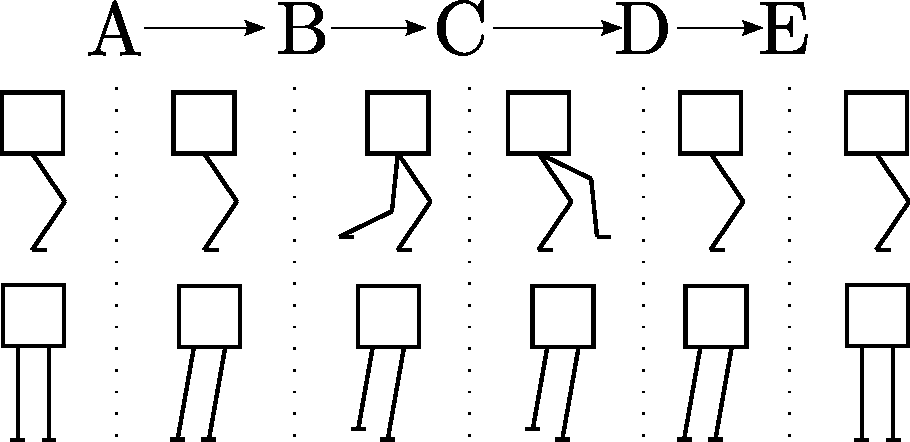
\includegraphics[width=0.7\textwidth]{Chapter5/kicking_phases.pdf} 
    \caption{Phases for a kick with right leg. The upper row shows poses looked from the right of the robot, while the lower one presents poses looked from the front. Extracted from \cite{MestradoManga}.}
    \label{fig:kicking_phases}
\end{figure}


\section{Metrics}
\label{sec:metrics}

When working on some reinforcement learning tasks, it is very important to previously define some metrics to assess the learning performance during the training stages. Raising this information, we can evaluate the techniques, identify the problems and consider improvements. In this work, we focused on two main metrics:

\begin{itemize}
\item \textbf{Episode accumulated reward:} Maximizing the episode return is the ultimate goal of RL, and therefore it is the most obvious performance indicator, providing a very good sense of how well the agent's actions are doing.

\item \textbf{Data efficiency:} A quantitative measure of how long, or how much data, an agent takes to learn a good behavior.
\end{itemize}

We calculate all these metrics in an offline manner, by logging all the state and action information from the agent during the training procedure.


